\documentclass[handout]{beamer}


\usetheme{default}
\usepackage{subfigure}
\usepackage{Sweave}
\usepackage{graphicx}
\usepackage{color}
\usepackage{multicol}
\usepackage{bm}


\author{Patrick Lam}
\title{A Brief Review of Probability}
\date{}
%\date{September 22, 2008}

\begin{document}

\newcommand{\red}{\textcolor{red}}
\newcommand{\blue}{\textcolor{blue}}
\newcommand{\purple}{\textcolor{purple}}

\frame{\titlepage}

\begin{frame}
\frametitle{Outline}
\tableofcontents
\end{frame}



\section{Expectation, Variance, and Densities}


\begin{frame}
\frametitle{Outline}
\tableofcontents[currentsection]
\end{frame}

\begin{frame}
\frametitle{Expectation}
\pause
The expected value of a random variable $X$ is simply the weighted
average of all possible values of $X$.\\
\bigskip
\pause
Discrete Case:
\pause
\begin{eqnarray*}
E(X) = \sum_i x_i P(X = x_i)
\end{eqnarray*}
where $P(X = x)$ is the probability mass function (PMF).\\
\pause
\bigskip
Continuous Case:
\pause
\begin{eqnarray*}
E(X) = \int^{\infty}_{-\infty} x p(x) dx
\end{eqnarray*}
where $p(x)$ is the probability density function (PDF).
\end{frame}

\begin{frame}
\frametitle{Expectation of a Function of a Random Variable}
\pause
Suppose we want to find $E[g(X)]$, where $g(X)$ is any function of
$X$.  \pause  We can simply weight the values of $g(x)$ by the PDF or
PMF of $X$:
\pause
\begin{eqnarray*}
E[g(X)] = \sum_i g(x_i) P(X = x_i)
\end{eqnarray*}
for discrete random variables \pause and 
\begin{eqnarray*}
E[g(X)] = \int_{-\infty}^{\infty} g(x) p(x) dx
\end{eqnarray*}
for continuous random variables.  \\
\bigskip
\pause
This is sometimes known as the \textit{Law of the Unconscious
Statistician} (LOTUS).
\end{frame}

\begin{frame}
\frametitle{Variance}
\pause
The formula for the variance of a random variable is 
\begin{eqnarray*}
\mathrm{Var}(X) = E[(X - E(X))^2]
\end{eqnarray*}
\pause
We can find the variance using LOTUS, \pause or we can simplify the
formula first.
\pause
\begin{eqnarray*}
\mathrm{Var}(X) &=& E[(X - E(X))^2]\\
\pause
&=& E[X^2 - 2 X E(X) + (E(X))^2]\\
\pause
&=& E(X^2) - 2 E(X) E[E(X)] + E([E(X)]^2)\\
\pause
&=& E(X^2) - 2 [E(X)]^2 + [E(X)]^2\\
\pause
&=& \mathbf{E(X^2) - [E(X)]^2}
\end{eqnarray*}
\pause
We can then find the first part with LOTUS.
\end{frame}

\begin{frame}
\frametitle{Marginal, Conditional, and Joint Densities}
\pause
\begin{eqnarray*}
p(x) &=& \int p(x,y) dy\\
\pause
p(x,y) &=& \int p(x,y,z) dz\\
\pause
p(x|y) &=& \frac{p(x,y)}{p(y)}\\
\pause
p(x|y,z) &=& \frac{p(x,y,z)}{p(y,z)}\\
\pause
p(x,y) &=& p(x | y) p(y)\\
\pause
&=& p(y | x) p(x) \\
\pause
p(x,y,z) &=& p(x | y,z) p(y|z) p(z)
\end{eqnarray*}
\end{frame}



\section{Important Distributions}


\begin{frame}
\frametitle{Outline}
\tableofcontents[currentsection]
\end{frame}

\subsection{Discrete Distributions}


\begin{frame}
\frametitle{Outline}
\tableofcontents[currentsubsection]
\end{frame}

\begin{frame}
\frametitle{The Bernoulli Distribution}
\begin{multicols}{2}
\pause
$Y \sim$ Bernoulli$(\pi)$\\
\bigskip
\pause
$y = 0,1$\\
\bigskip
\pause
probability of success: $\pi \in [0,1]$\\
\bigskip
\pause
$p(y|\pi) = \pi^y (1 - \pi)^{(1-y)}$\\
\bigskip
\bigskip
\pause
$E(Y) = \pi$\\
\bigskip
\pause
Var$(Y) = \pi (1 - \pi)$
\pause


\begin{figure}[!htp]
\begin{center}
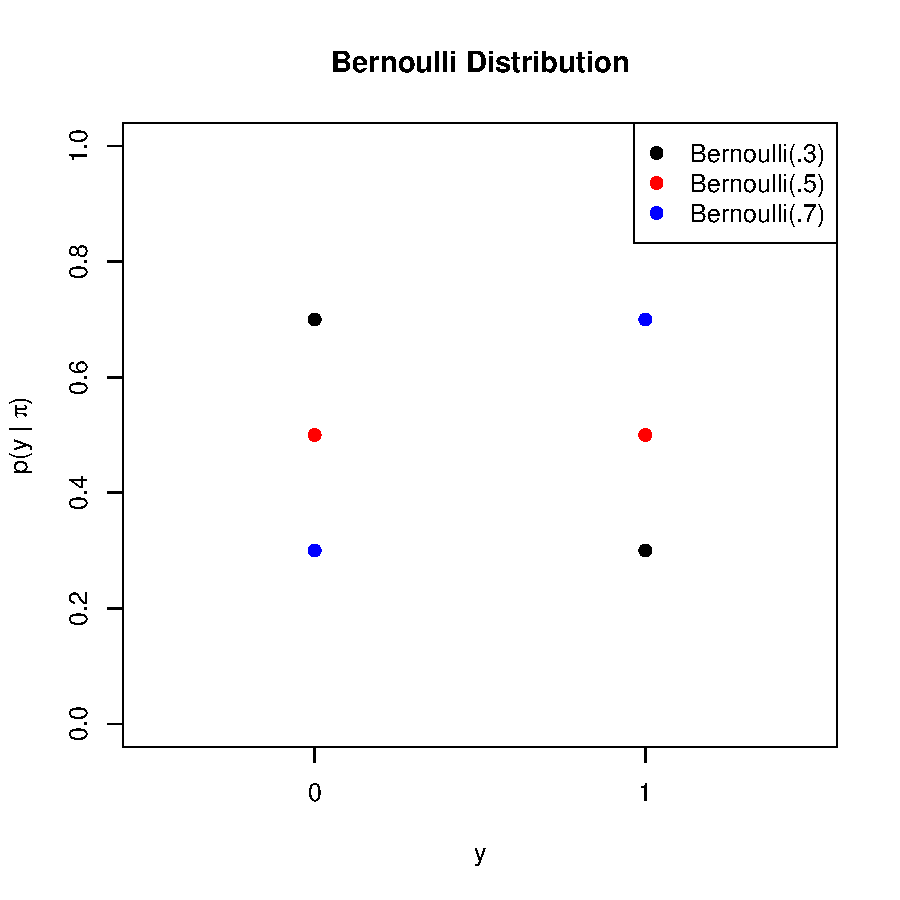
\includegraphics[width=2in, height=2in]{probability-bernoulli.pdf}
\end{center}
\end{figure}
\end{multicols}
\end{frame}



\begin{frame}
\frametitle{The Binomial Distribution}
\begin{multicols}{2}
\pause
$Y \sim$ Binomial$(n, \pi)$\\
\bigskip
\pause
$y = 0,1,\dots,n$\\
\bigskip
\pause
number of trials: $n \in \{1,2,\dots \}$\\
\pause
probability of success: $\pi \in [0,1]$\\
\bigskip
\pause
$p(y|\pi) = \binom{n}{y} \pi^y (1 - \pi)^{(n-y)}$\\
\bigskip
\bigskip
\pause
$E(Y) = n \pi$\\
\bigskip
\pause
Var$(Y) = n \pi (1 - \pi)$
\pause


\begin{figure}[!htp]
\begin{center}
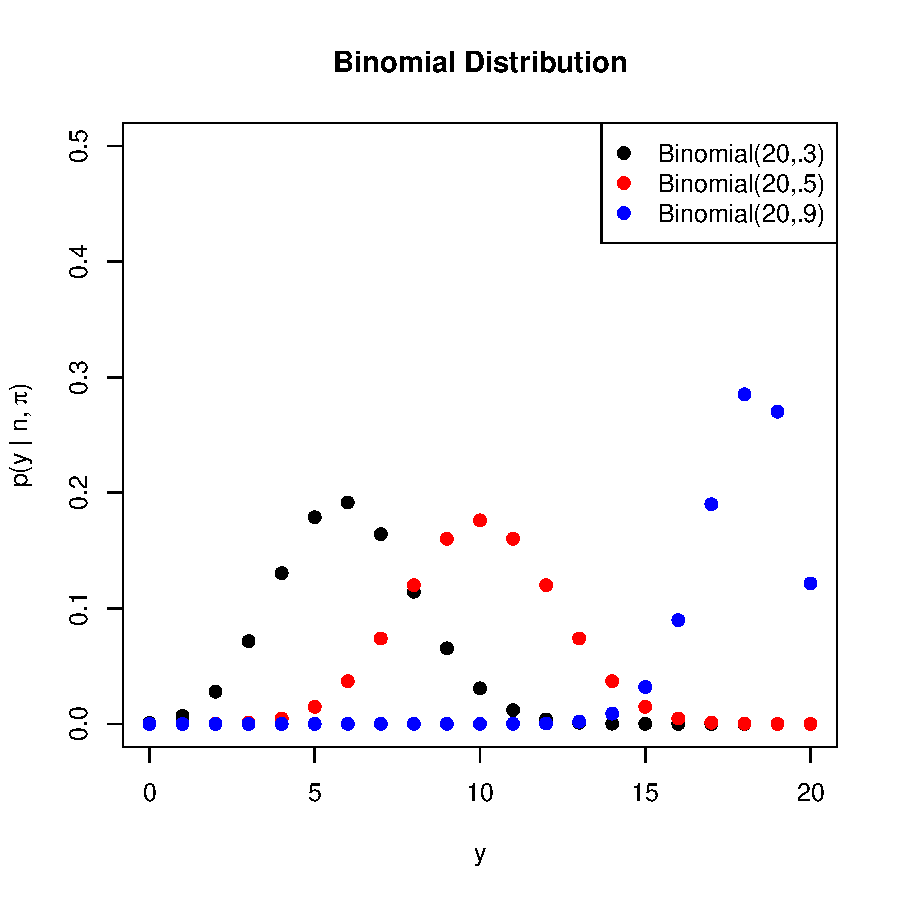
\includegraphics[width=2in, height=2in]{probability-binomial.pdf}
\end{center}
\end{figure}
\end{multicols}
\end{frame}


\begin{frame}
\frametitle{The Multinomial Distribution}
\pause
$Y \sim$ Multinomial$(n,\pi_1, \dots, \pi_k)$\\
\bigskip
\pause
$y_j = 0,1,\dots,n; \; \; \sum_{j=1}^k y_j = n$\\
\bigskip
\pause
number of trials: $n \in \{1,2,\dots \}$\\
\pause
probability of success for $j$: $\pi_j \in [0,1]; \; \; \sum_{j=1}^k
\pi_j = 1$\\
\bigskip
\pause
$p(\mathbf{y}|n,\bm{\pi}) = \frac{n!}{y_1! y_2! \dots
y_k!}\pi_1^{y_1}\pi_2^{y_2} \dots \pi_k ^ {y_k}$\\
\bigskip
\bigskip
\pause
$E(Y_j) = n\pi_j$\\
\bigskip
\pause
Var$(Y_j) = n \pi_j (1 - \pi_j)$\\
\bigskip
\pause
Cov$(Y_i, Y_j) = -n \pi_i \pi_j$


\end{frame}



\begin{frame}
\frametitle{The Poisson Distribution}
\begin{multicols}{2}
\pause
$Y \sim$ Poisson$(\lambda)$\\
\bigskip
\pause
$y = 0,1,\dots$\\
\bigskip
\pause
expected number of occurrences: $\lambda > 0$\\
\bigskip
\pause
$p(y|\lambda) = \frac{e^{-\lambda} \lambda^y}{y!}$\\
\bigskip
\bigskip
\pause
$E(Y) = \lambda$\\
\bigskip
\pause
Var$(Y) = \lambda$
\pause


\begin{figure}[!htp]
\begin{center}
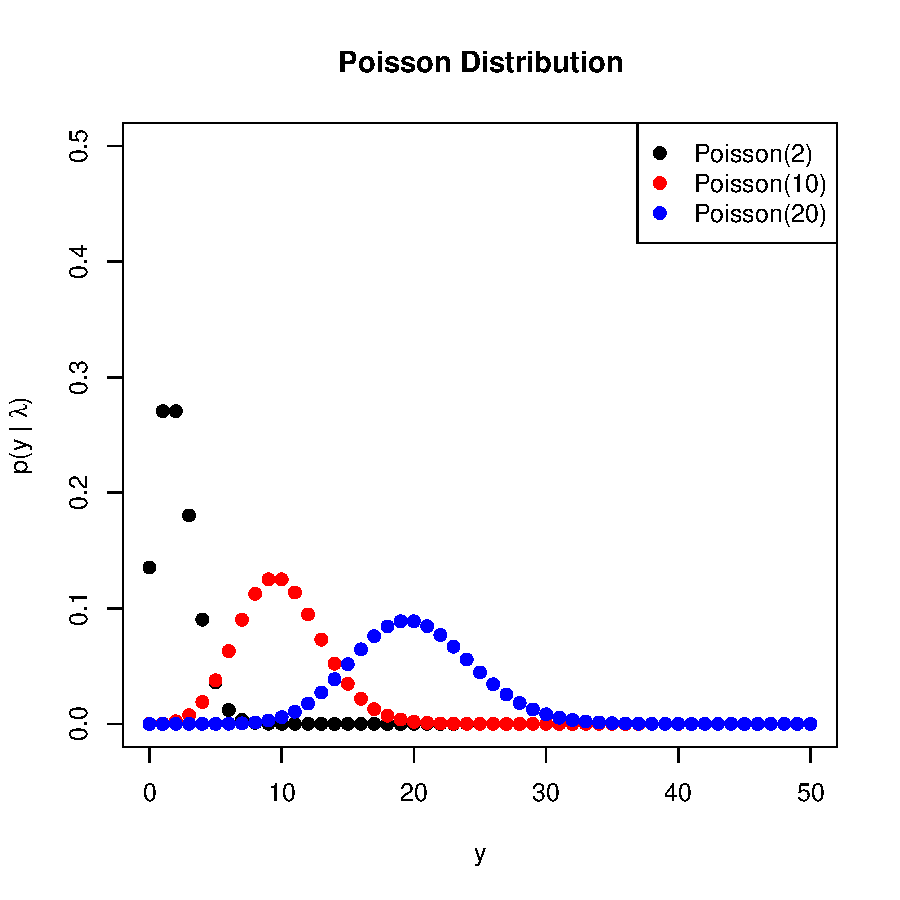
\includegraphics[width=2in, height=2in]{probability-poisson.pdf}
\end{center}
\end{figure}
\end{multicols}
\end{frame}

\begin{frame}
\frametitle{The Geometric Distribution}
\pause
How many Bernoulli trials until success?
\begin{multicols}{2}
\pause
$Y \sim$ Geometric$(\pi)$\\
\bigskip
\pause
$y = 1,2,3,\dots$\\
\bigskip
\pause
probability of success: $\pi \in [0,1]$\\
\bigskip
\pause
$p(y|\pi) = (1 - \pi)^{(y-1)} \pi$\\
\bigskip
\bigskip
\pause
$E(Y) = \frac{1}{\pi}$\\
\bigskip
\pause
Var$(Y) = \frac{1 - \pi}{\pi^2}$
\pause


\begin{figure}[!htp]
\begin{center}
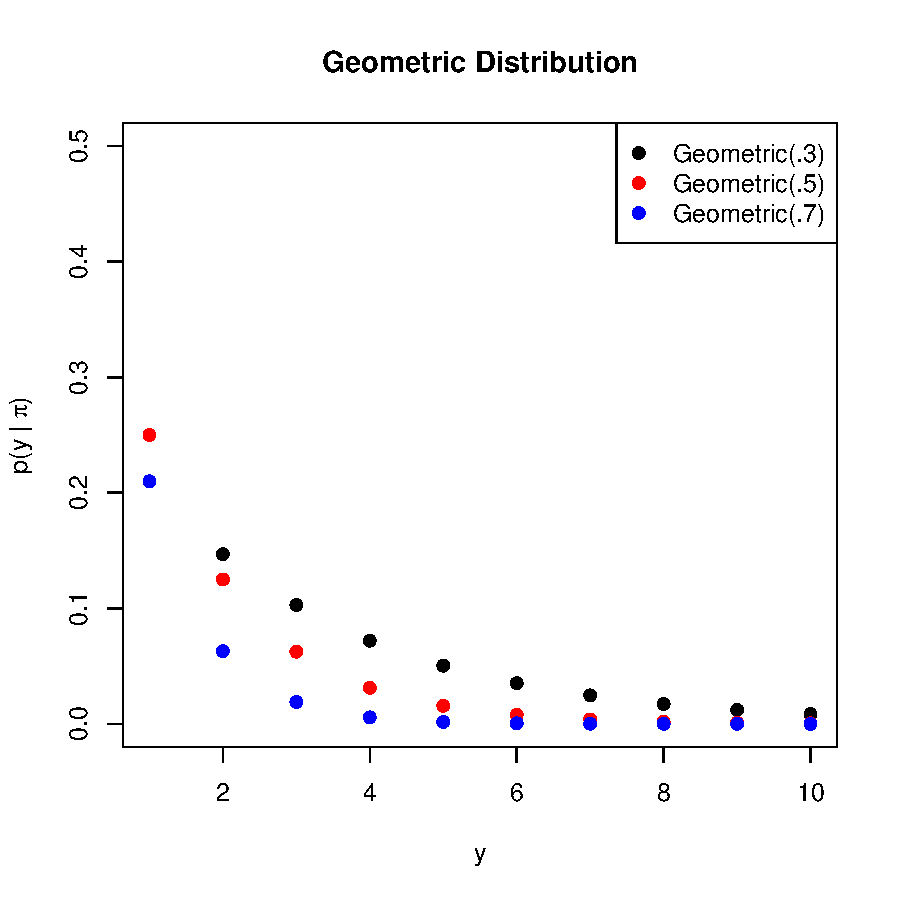
\includegraphics[width=2in, height=2in]{probability-geometric.pdf}
\end{center}
\end{figure}
\end{multicols}
\end{frame}

\subsection{Continuous Distributions}


\begin{frame}
\frametitle{Outline}
\tableofcontents[currentsubsection]
\end{frame}

\begin{frame}
\frametitle{The Univariate Normal Distribution}
\begin{multicols}{2}
\pause
$Y \sim$ Normal$(\mu, \sigma^2)$\\
\bigskip
\pause
$y \in \mathbb{R}$\\
\bigskip
\pause
mean: $\mu \in \mathbb{R}$\\
\pause
variance: $\sigma^2 > 0$\\
\bigskip
\pause
$p(y|\mu, \sigma^2) = \frac{\exp \left( {-\frac{(y - \mu)^2}{2\sigma^2} } \right)}{\sigma \sqrt{2 \pi}}$\\
\bigskip
\bigskip
\pause
$E(Y) = \mu$\\
\bigskip
\pause
Var$(Y) = \sigma^2$
\pause


\begin{figure}[!htp]
\begin{center}
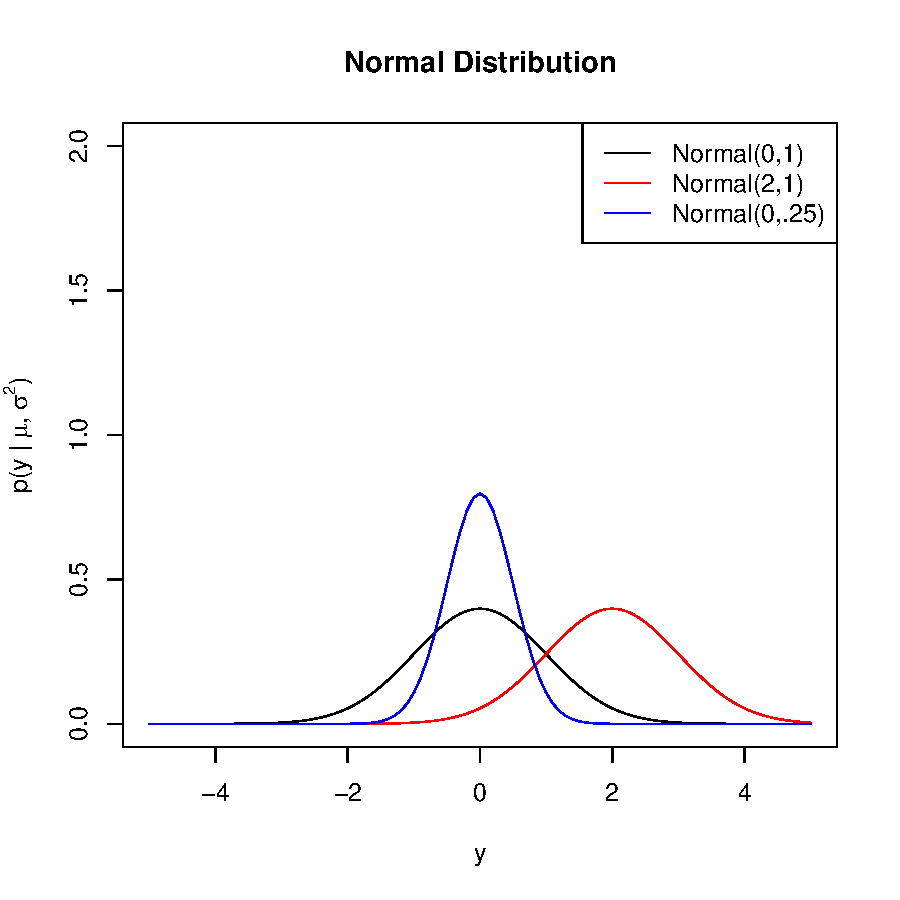
\includegraphics[width=2in, height=2in]{probability-normal.pdf}
\end{center}
\end{figure}
\end{multicols}
\end{frame}



\begin{frame}
\frametitle{The Multivariate Normal Distribution}
\pause
$Y \sim \mathcal{N}(\bm{\mu},\bm{\Sigma})$\\
\bigskip
\pause
$\mathbf{y} \in \mathbb{R}^k$\\
\bigskip
\pause
mean vector: $\bm{\mu} \in \mathbb{R}^k$\\
\pause
variance-covariance matrix: $\bm{\Sigma}$ positive definite $k \times
k$ matrix\\
\bigskip
\pause
$p(\mathbf{y}|\bm{\mu},\bm{\pi}) = (2\pi)^{-k/2} | \bm{\Sigma}
|^{-1/2} \exp{\left( -\frac{1}{2} (\bm{y} - \bm{\mu})'
\bm{\Sigma^{-1}} (\bm{y} - \bm{\mu}) \right)}$\\
\bigskip
\bigskip
\pause
$E(Y) = \bm{\mu}$\\
\bigskip
\pause
Var$(Y) = \bm{\Sigma}$\\
\end{frame}


\begin{frame}
\frametitle{The Uniform Distribution}
\pause
$Y \sim$ Uniform$(\alpha, \beta)$\\
\bigskip
\pause
$y \in [\alpha, \beta]$\\
\bigskip
\pause
Interval: $[\alpha, \beta]; \; \; \beta > \alpha$\\
\bigskip
\pause
$p(y| \alpha, \beta) = \frac{1}{\beta - \alpha}$\\
\bigskip
\bigskip
\pause
$E(Y) = \frac{\alpha + \beta}{2}$\\
\bigskip
\pause
Var$(Y) = \frac{(\beta - \alpha)^2}{12}$

\end{frame}



\begin{frame}
\frametitle{The Beta Distribution}
\begin{multicols}{2}
\pause
$Y \sim$ Beta$(\alpha, \beta)$\\
\bigskip
\pause
$y \in [0,1]$\\
\bigskip
\pause
shape parameters: $\alpha > 0; \; \; \beta > 0$\\
\bigskip
\pause
$p(y| \alpha, \beta) = \frac{\Gamma (\alpha + \beta)}{\Gamma (\alpha)
\Gamma (\beta)} y^{(\alpha - 1)} (1 - y)^{(\beta-1)}$\\
\bigskip
\bigskip
\pause
$E(Y) = \frac{\alpha}{\alpha + \beta}$\\
\bigskip
\pause
Var$(Y) = \frac{\alpha \beta}{(\alpha + \beta)^2 )\alpha + \beta + 1)}$


\begin{figure}[!htp]
\begin{center}
\includegraphics[width=2in, height=2in]{probability-beta.pdf}
\end{center}
\end{figure}
\end{multicols}

\end{frame}


\begin{frame}
\frametitle{The Gamma Distribution}
\pause
\begin{multicols}{2}
$Y \sim$ Gamma$(\alpha, \beta)$\\
\bigskip
\pause
$y > 0$\\
\bigskip
\pause
shape parameter: $\alpha > 0$\\
\pause
inverse scale parameter: $\beta > 0$ \\
\bigskip
\pause
$p(y| \alpha, \beta) = \frac{\beta^{\alpha}}{\Gamma (\alpha)}
y^{(\alpha - 1)} \exp{(-\beta y)}$\\
\bigskip
\bigskip
\pause
$E(Y) = \frac{\alpha}{\beta}$\\
\bigskip
\pause
Var$(Y) = \frac{\alpha}{\beta^2}$


\begin{figure}[!htp]
\begin{center}
\includegraphics[width=2in, height=2in]{probability-gamma.pdf}
\end{center}
\end{figure}
\end{multicols}
\end{frame}


\begin{frame}
\frametitle{The Inverse Gamma Distribution}
\pause
Distribution of the Inverse of a Gamma Distribution: \pause If $X \sim$
Gamma($\alpha, \beta$), then $\frac{1}{X} \sim$ Invgamma($\alpha, \beta$).
\begin{multicols}{2}
\pause
$Y \sim$ Invgamma$(\alpha, \beta)$\\
\bigskip
\pause
$y > 0$\\
\bigskip
\pause
shape parameter: $\alpha > 0$\\
\pause
scale parameter: $\beta > 0$\\
\bigskip
\pause
$p(y|\alpha, \beta) = \frac{\beta^\alpha}{\Gamma(\alpha)}
y^{-(\alpha+1)} e^{-\frac{\beta}{y}}$\\
\bigskip
\bigskip
\pause
$E(Y) = \frac{\beta}{\alpha-1}$ for $\alpha > 1$\\
\bigskip
\pause
Var$(Y) = \frac{\beta^2}{(\alpha-1)^2 (\alpha-2)}$ for $\alpha > 2$
\pause


\begin{figure}[!htp]
\begin{center}
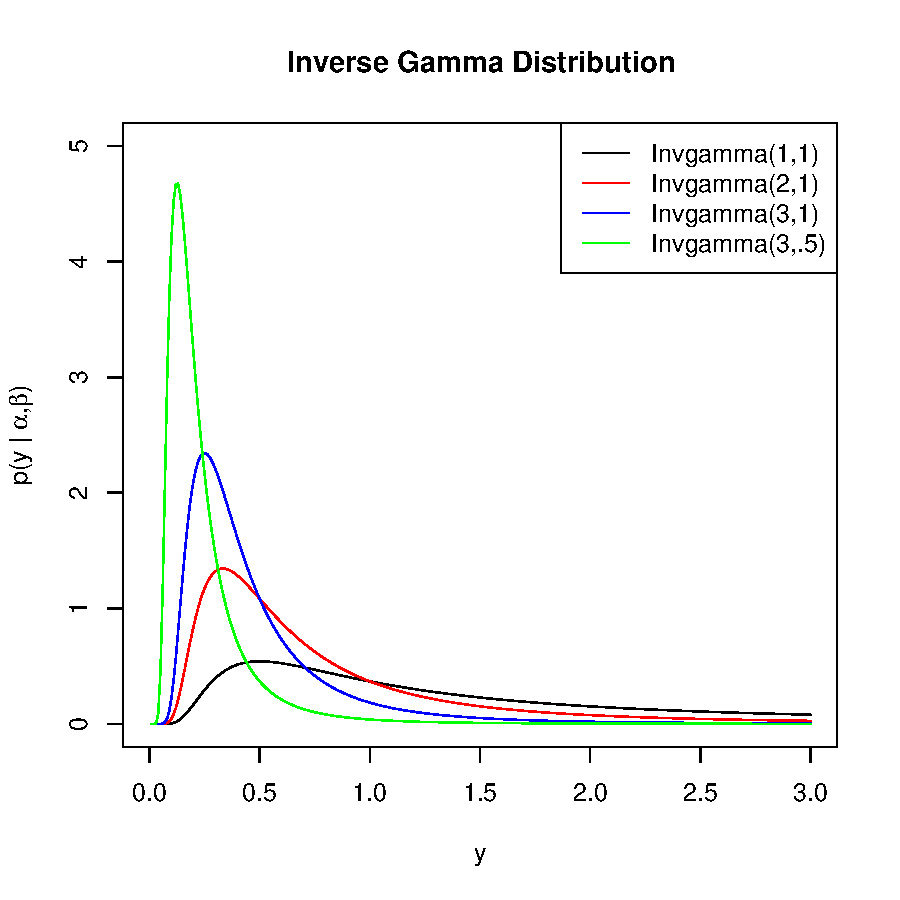
\includegraphics[width=2in, height=2in]{probability-invgamma.pdf}
\end{center}
\end{figure}
\end{multicols}
\end{frame}


\begin{frame}
\frametitle{The Dirichlet Distribution}
\pause
$Y \sim$ Dirichlet$(\alpha_1,\dots, \alpha_k)$\\
\bigskip
\pause
$y_j \in [0,1]; \; \; \sum_{j=1}^{k} y_j = 1$\\
\bigskip
\pause
$\alpha$ parameters: $\alpha_j > 0; \; \; \sum_{j=1}^k \alpha_j \equiv
\alpha_0$\\
\bigskip
\pause
$p(\mathbf{y}| \bm{\alpha}) = \frac{\Gamma (\alpha_1 + \dots +
\alpha_k)}{\Gamma (\alpha_1) \dots \Gamma (\alpha_k)} y_1^{\alpha_1 -
1} \dots y_k^{\alpha_k - 1}$\\
\bigskip
\bigskip
\pause
$E(Y_j) = \frac{\alpha_j}{\alpha_0}$\\
\bigskip
\pause
Var$(Y_j) = \frac{\alpha_j (\alpha_0 - \alpha_j)}{\alpha^2_0 (\alpha_0
+ 1)}$\\
\bigskip
\pause
Cov$(Y_i, Y_j) = -\frac{\alpha_i \alpha_j}{\alpha^2_0 (\alpha_0 + 1)}$
\end{frame}

\end{document}
